\documentclass[12pt,fleqn]{article}
\setlength{\parindent}{0pt}
\usepackage{graphicx}
\usepackage{cancel}
\usepackage{listings}
\usepackage[latin5]{inputenc}
\usepackage{color}
\setlength{\parskip}{8pt}
\setlength{\parsep}{0pt}
\setlength{\headsep}{0pt}
\setlength{\topskip}{0pt}
\setlength{\topmargin}{0pt}
\setlength{\topsep}{0pt}
\setlength{\partopsep}{0pt}
\setlength{\mathindent}{0cm}

\begin{document}
MIT OCW Cok Degiskenli Calculus - Ders 19

Konumuz vektor alanlari (vector fields) ve cizgi entegralleri (line
integrals). Bundan onceki derslerde cift entegral (double integral)
konusunu isledik, fakat o tur entegraller cizgi entegrallerinden tamamen
farklidir, yani bu dersi takip ederken cift entegraller ile baglantilari
dusunmemek daha iyi olur, kafalar karismasin. 

Vektor Alanlari

Vektor alanlari bir vektordurler aslinda, diyelim ki $\vec{F}$

\[ \vec{F} = M\hat{i} + N\vec{j} \]

Farkli olan $M,N$ kendilerinin $x,y$'nin bir fonksiyonu olmalaridir. Bu
demektir ki kordinat sistemindeki her $x,y$ kombinasyonu icin degisik bir
vektor olacaktir. Bir misir tarlasinda her noktada misir vardir, vektor
alaninda her noktada bir vektor vardir [hoca bu analojiyi misirlar uzun,
yonleri olan seyler oldugu icin kullaniyor herhalde]. Daha once
$\vec{r}(t)$ baglaminda $t$ degiskenine bagliligi gorduk, fakat o tek
degisken idi, zaten bir egriyi vektor ile temsil etmek icin oyle olmasi
gerekiyordu, burada birden fazla degisken $x,y$'ye bagimlilik var. 

Bu kavram bir sivi, bir ruzgar icindeki akis vektorlerini temsil etmek icin
kullanilabilir mesela. Ya da kuvvet alani (force field) kavrami -- bu
kavram Star Wars filminden bir kavram degil. Yeryuzunde elimizde bir cismi
herhangi bir yerde tuttugumuzda onun uzerinde etki eden bir kuvvet vektoru
var, bu vektor her noktada degisik, ve tum bu vektorlerin toplami bir
kuvvet alani olusturuyorlar, ki bualan bir vektor alanidir. 

Biz bu derste konuya pur matematiksel olarak bakiyoruz, sadece arka
plandaki bu fiziksel baglantiyi motivasyon acisindan aklimizda
tutabiliriz. 

Once cizimden baslayalim

Ornek

\[ \vec{F} = 2\hat{i} + \hat{j} \]

Tam $x,y$'ye baglantidan bahsetmistik, baglantisiz bir tane verdik! Ama
ornegi soyle gorebiliriz, bu alan her $x,y$ icin ayni vektore sahip. Yani
yine $x,y$'yi merkez alarak dusunuyoruz, sadece vektorun her noktada ayni
oldugunu soylemis oluyoruz.

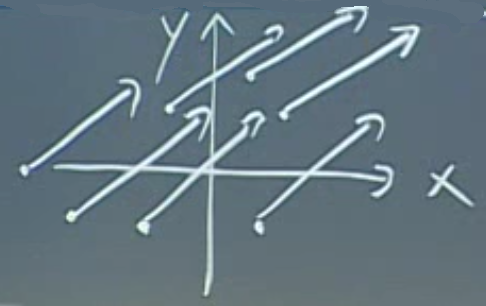
\includegraphics[height=4cm]{19_1.png}

Ornek

\[ \vec{F} = x\hat{i} \]

Y-ekseni uzerinde, yani $x$'in sifir oldugu noktada (zaten hic $y$ yok)
vektor sifir buyuklugunde. Diger noktalarda vektor yatay, $x$ buyudukce, ya
a eksi yonde kuculdukce, saga ya da sola dogru vektorun buyuklugu de
degisecek.

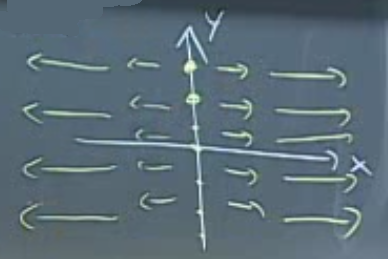
\includegraphics[height=4cm]{19_2.png}

Aslinda bu tur cizimleri cogunlukla bilgisayara yaptiriyoruz, ama kabaca
vektor alanlarinin neye benzedigini hayal edebilmek ise yariyor. 

Ornek

\[ \vec{F} = x\hat{i} + y\hat{j} \]

Bu alanin ilginc bir geometrik sonucu var.  Orijinden herhangi bir noktaya
cizilebilecek bir vektoru (... ile belirtiliyor) alip, kopyalarsak, bu
kopyayi o noktadan baslayacak sekilde yerlestirirsek, dogru sonucu elde
etmis oluruz.

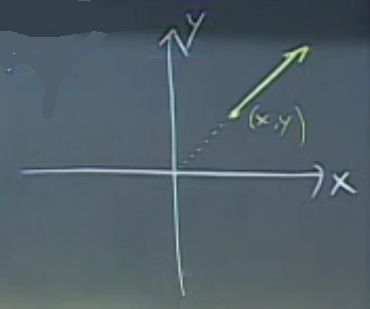
\includegraphics[height=4cm]{19_3.png}













\end{document}
